\chapter{Gestión de Proyectos}

Scrum puede verse como un marco ágil de gestión de proyectos para el desarrollo incremental de productos, valiéndose de equipos autoorganizados. 



\subsection{Proyecto Scrum}

Un proyecto, en ingeniería de software, es un esfuerzo temporal que se lleva a cabo para crear un sistema, software o resultado único\footnote{Se parafrasea la definición del PMBOOK \cite{PMBOK-2004}.}. Los proyectos son organizados, en una empresa u organización, por el proceso de administración de proyectos. Según este proceso, el ciclo de vida de los proyectos se puede dividir en tres fases: inicio, ejecución y cierre (ver figura \ref{fig:PMIProject}). 

\subsection{Planificación}

En la administración de proyectos es necesario planificar y dicha actividad se suele hacer en la fase de inicio ("Starting phase" o "Project Start"). Pero, a diferencia de la metodología clásica (ver figura \ref{fig:PMIProject}) en que la planificación estaba siempre al inicio y el desarrollo en la fase de ejecución, en el marco Scrum la planificación se distribuye durante todo el ciclo de vida del proyecto y en la fase de ejecución se hace el desarrollo incremental de productos (por incrementos de producto) en iteraciones cortas (Sprint) donde cada iteración tiene su respectiva planificación (ver figura \ref{fig:ScrumProject}) y su incremento de producto, en caso de haberlo logrado (idealmente producto integrado y funcionando de cara al usuario o cliente).

\begin{figure}[h]
  \centering
  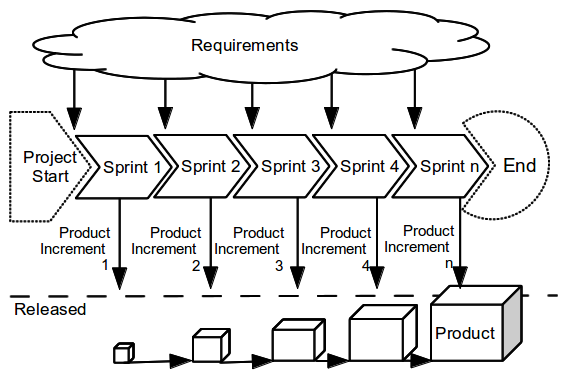
\includegraphics[width=0.90\textwidth]{ScrumProject}
  \caption{Proyecto Scrum}
  \centering
  \label{fig:ScrumProject} %\ref{fig:ScrumProject}
\end{figure}

Entonces podemos decir que en Scrum se piensa en muchos planes periódicos (a corto plazo). Los mismo pueden estar en un plan mayor a largo plazo pero de carácter flexible. También se puede realizar un plan global de entregables en base a los incrementos de producto estimados. Pero, desde esta perspectiva, hay que considerar que aunque se trabaje con planificaciones, los planes no son contratos a respetar a rajatabla.

\subsubsection{Inicio de proyecto}

En la etapa de inicio de proyecto ("Project Start") se puede hacer una “inception”, aunque esta técnica no es parte de Scrum. En una inception se hace un plan versátil alto nivel a corto plazo (un roadmap o release plan) para poder guiar e iniciar el desarrollo bajo el esquema Scrum.

%Triangle of Project Management
\subsection{Triángulo de la Gestión de proyectos}

El marco de Scrum cambia el triángulo clásico de la gestión de proyectos. El compromiso ya no es entre el tiempo, presupuesto y calidad; sino que se basa en el triángulo de: Presupuesto (Costo), Tiempo y funcionalidad (alcance) (ver figura \ref{fig:ScrumProjectManagementTriangle}). Además, tradicionalmente se ha intentado fijar el alcance para negociar y variar el presupuesto y el tiempo. En cambio, desde la agilidad, se intenta mantener fijos el tiempo y el presupuesto mientras se varía el alcance\footnote{\cite{Martin-Alaimo-2014}}. La pregunta habitual es: ¿cuánto puedes hacer en este tiempo (bajo un costo fijo)?
La ventaja de esta aproximación es que en vez de focalizarnos en plazos con fechas de entrega, nos centramos en desarrollar valor. ¿Cual es el máximo valor que podemos desarrollar en un tiempo dado?

\begin{figure}[h]
  \centering
  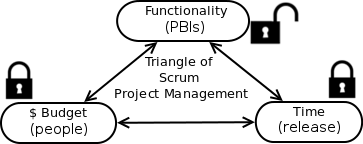
\includegraphics[width=0.60\textwidth]{ScrumProjectManagementTriangle}
  \caption{Triángulo de Gestión de Proyectos Scrum}
  \centering
  \label{fig:ScrumProjectManagementTriangle} %\ref{fig:ScrumProjectManagementTriangle}
\end{figure}

\subsection{Planificación de entregables}

Con este marco de trabajo tampoco es necesario hacer una entrega final (o "releasing") ya que se pueden hacer entregas paulatinas. En cada sprint se puede entregar valor. Para hacer entregas intermedias planificadas se puede crear un plan de muy alto nivel para múltiples Sprints durante una planificación de lanzamientos (por ejemplo en una inception) llamado "Release Plan". Este plan de entregables o de lanzamientos es una guía con la que se pretende reflejar las expectativas sobre qué funcionalidad se implementará y cuándo, aproximadamente, se completará \footnote{\cite{Scrum-Institute-2015}}. También sirve como una base para monitorear el progreso dentro del proyecto. Pero siempre hay que considerar que no es un plan equivalente a un plan clásico, los hitos de releases no deberían ser compromisos rígidos y contractuales y, además, el desarrollo del proyecto no debería centrarse en respetar el plan. Por este motivo el plan de lanzamiento no es un plan estático; pues, se cambia durante todo el proyecto cuando nuevos requerimientos o conocimientos están disponible y, por ejemplo, cuando entradas en el Scrum Product Backlog cambian y se re-estiman. Por lo tanto, este plan debe ser revisado y actualizado en intervalos regulares, por ejemplo, después de cada Sprint.

\subsubsection{Release Plan Ágil}

Un "Release Plan" ágil es, normalmente, un conjunto de historias de usuario (o épicas) agrupadas por "releases" o versiones del producto que se ponen a disposición de los usuarios \footnote{Release plan, jmbeas, 2011; Agile Estimating and Planning, Mike Cohn}. En otras palabras, es una planificación a media distancia como una proyección hacia adelante en una serie de sprints \footnote{Release Planning, Retiring the Term but not the Technique, Mike Cohn, 2012.}. Esta planificación es algo valiosa de hacer cuando se usa el marco Scrum, pero no es requerido por el "núcleo Scrum" o el "Scrum originario" \footnote{Gone are Release Planning and the Release Burndown, Ralph Jocham and Henk Jan Huizer in Community Publications, Scrum.org, Saturday, October 01, 2011; Ken Schwaber and Jeff Sutherland Release Updated Scrum Guide, David Bulkin, Infoq.com on Jul 27, 2011}. Se puede utilizar Scrum con éxito sin necesidad de utilizar “Release Planning”.

Hay que remarcar que bajo el marco Scrum, si se hace un Release Plan, debería ser un documento minimalista (buscando el principio de simplicidad), pensado para MVPs (producto de mínimo valor) o entregas frecuentes (respetando el valor de software funcionando), abierto a modificaciones constantes (adaptabilidad y desarrollo evolutivo), consensuado con el equipo (transparencia) y desarrollado por el PO en colaboración con el cliente y con el equipo de desarrollo (priorizando la conversación y no la relación contractual).

Luego hay que tener en cuenta que para crearlo se deben tener disponibles las siguientes cosas:

\begin{enumerate}
\item Un Product Backlog priorizado y estimado.
\item La velocidad estimada del Equipo Scrum.
\item Las condiciones de satisfacción (metas para la agenda, el alcance, los recursos) o impacto deseado.
\end{enumerate}

\subsection{Gestión de proyecto orientada a producto}

El verdadero objetivo de Scrum es conseguir un producto mínimo viable o MVP en manos de los futuros clientes cuán rápido sea posible y obtener sus comentarios como feedback temprano\footnote{\cite{Jeff-Sutherland-2016}}. MVP es una estrategia para el aprendizaje de forma iterativa sobre sus clientes para poner a prueba las hipótesis fundamentales del negocio \footnote{\cite{Greg-Gehrich-2012}}. Es un incremento de producto, subconjunto del 20\% de features que representan parte del 80\% de valor\footnote{\cite{Jeff-Sutherland-2016}}. Las features del MVP representan conceptualmente al producto final completo y se prueba con un grupo de usuarios "early adopters". Las pruebas deben ser medibles y se hacen sobre las hipótesis fundamentales del producto como negocio.

Por otro lado hay otro concepto que se maneja en el ámbito de la agilidad, el MMP (Minimal Marketable Product). El MMP es el producto con el más pequeño posible conjunto de features y que crea la experiencia del usuario deseada, y por lo tanto puede ser comercializado y vendido, tempranamente, con éxito.

Resumidamente, la gestión de proyecto se orienta al producto y su ciclo de vida. Un producto puede evolucionar mediante una secuencia de releases, de los cuales algunos entregan valor directamente de cara al público. Después de una etapa de creatividad y prototipado (si el producto es nuevo y/o novedoso), tendremos uno o una secuencia de entregables MVPs hasta llegar a un MMP, que será el mínimo producto que se lanza al mercado como tal. De allí en adelante comienza el crecimiento en escalamiento (Growth) e incremento de funcionalidad hasta alcanzar una madurez (maturity), para finalmente constituir un producto final estable o commodity (ver fig. \ref{fig:product_evolution})\footnote{\cite{Greg-Gehrich-2012}}.

\begin{figure}[h]
  \centering
  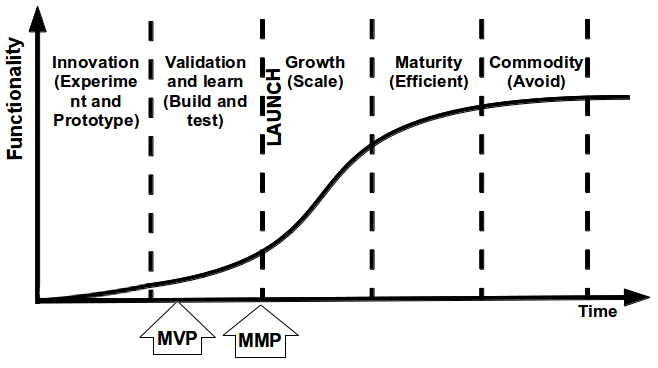
\includegraphics[width=0.70\textwidth]{product_evolution}
  \caption{Crecimiento del producto}
  \centering
  \label{fig:product_evolution} %\ref{fig:product_evolution}
\end{figure}

\subsection{Gestión de riesgos}

Si bien la gestión de riesgos no es parte de scrum y un facilitador no se encarga de la gestión al modo tradicional como la gestión de riesgos, sí debería velar por mitigar los problemas que surjan en el proyecto y apoyar, en consecuencia, a la gestión de riesgos. En este sentido, no solo se encargaría de ayudar a desbloquear problemas y reducir impedimentos para que el sistema de trabajo fluya, sino que también puede preocuparse de prever issues para anticiparse a los problemas y controlar así, de antemano y en la medida de lo posible, los riesgos asociados a bloqueos del flujo de trabajo que atentan contra los objetivos del proyecto. Lo difícil es lograr una gestión de riesgos ágil en vez de una gestión pesada, dificultosa y que demande mucho esfuerzo de gestión. En esta vía, es preferible mantener un simple registro de riesgos con información concisa. Los datos principales a registrar de un riesgo, además de su nombre, pueden ser: descripción, probabilidad (probability), impacto (severity), criticidad (criticality), acciones de mitigación, dueño y estado.

Algo simple que se puede lograr trabajando con criticidad es usar tres valores en la probabilidad de ocurrencia y en el impacto (1, 2 y 3). El impacto representa la severidad de la ocurrencia de un problema asociado al riesgo o el tiempo perdido (size of loss). Por otro lado, la criticidad representa la prioridad del riesgo o el grado en que ese riesgo afecta negativamente al proyecto (exposure). El mismo será resultado del producto entre la probabilidad y el impacto. En consecuencia, la criticidad podría ser: 1, 2, 3, 4, 6, 9.

\begin{figure}[h]
  \centering
  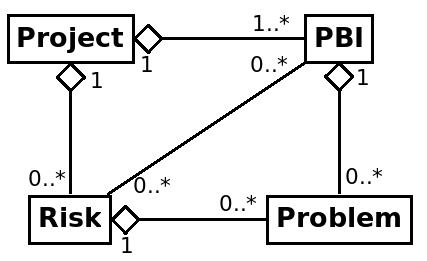
\includegraphics[width=0.40\textwidth]{RiskProblemDiagram}
  \caption{Diagrama de riesgos, problemas e ítems del proyecto (PBIs).}
  \centering
  \label{fig:RiskProblemDiagram} %\ref{fig:RiskProblemDiagram}
\end{figure}

Las herramientas gráficas que se pueden usar para dar visibilidad de los riesgos son: a) la “matriz de riesgos”; b) el “histórico de criticidad”; c) o el gráfico de curva de riesgo quemado (Risk Burn-down Chart).

La gestión de riesgos no es independiente de la gestión de impedimento o de problemas (issues o problem). Muchos de los problemas surgidos en el proyecto están asociados a riesgos identificados. Por tal motivo, la gestión de riesgos es útil, porque podemos mitigar los problemas de antemano. Por dicha razón, puede ser valioso llevar un registro de los issues y su relación con los riesgos. Siempre sin perder de vista no caer en el énfasis de la documentación ni en el afán de reportar. Se debe buscar la simplicidad y el foco en el flujo de trabajo sin impedimentos.

\begin{figure}[h]
  \centering
  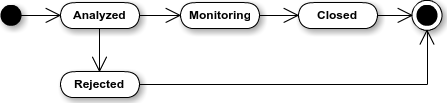
\includegraphics[width=0.70\textwidth]{RiskFlowDiagram}
  \caption{Estados posibles de un riesgo.}
  \centering
  \label{fig:RiskFlowDiagram} %\ref{fig:RiskFlowDiagram}
\end{figure}

Las herramientas gráficas útiles para dicha gestión son: “Tablero de Obstáculos” (obstacle board) o el "Calendario de Obstáculos" (Issues calendars).

\chapter{Métricas}
%\subsection{Métricas}

¿Para qué medir? Si no medimos no podemos adaptarnos bajo un marco empírico como propone Scrum. Medimos en forma transparente, en procesos de inspección y adaptación. Las métricas ayudan al equipo a medir su propio desempeño en el proceso de trabajo para poder hacer cambios basados en hechos. También es un soporte a la gestión de proyecto/producto para poder medir el progreso en cuanto a impacto de negocio (no a seguir un plan), tomar decisiones de negocio, revisar la productividad de valor y el desempeño\footnote{Las métricas se pueden usar para medir desempeño, pero no se deben utilizar en forma punitiva ni tampoco en sistemas de evaluación de desempeño de empleados.} del equipo en cuanto a madurez. Además hay indicadores de calidad de producto que nos pueden indicar aspectos claves de prestancia y salud de un producto. Se puede ver a las métricas como parte del monitoreo de salud del equipo, del sistema de trabajo, del producto y negocio; y parte del sistema de estabilización de la empresa y del sistema de mejora continua.

En síntesis, se pueden categorizar a las métricas en cuatro aspectos: trabajo en equipo (team), proceso de trabajo (process), calidad de producto (quality) e impacto de negocio (Impact) [ver fig. \ref{fig:Metrics_KPIs}].

\begin{figure}[h]
  \centering
  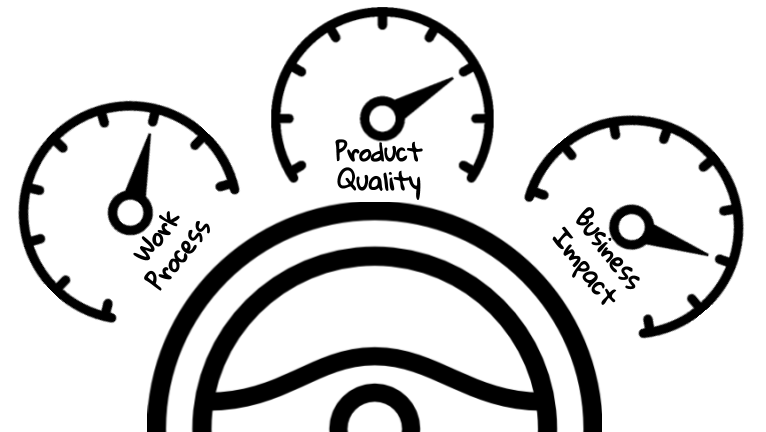
\includegraphics[width=0.85\textwidth]{Metrics_KPIs}
  \caption{Modelo de 4 categoría de métricas o KPIs.}
  \centering
  \label{fig:Metrics_KPIs} %\ref{fig:Metrics_KPIs}
\end{figure}
\FloatBarrier % Command to control the position of floating images. With its, I can get the figures not to be pushed to the end of the document.
% El comando FloatBarrier es usado aqui para que la imagen se clave en este lugar y que no sea acarreada al final del documento.

\subsection{Métricas de equipo}

El trabajo colaborativo es uno de los cuatro aspectos claves de la agilidad. Por tal motivo podemos medirlo de alguna manera simple para ayudar en la mejora contínua del equipo. A continuación puedo mostrar algunas sugerencias.

\begin{enumerate}

\item {\textbf{Team Happiness:}
Un estudio de Harvard muestra que la felicidad aumenta la producción de cualquier tipo de trabajo, pues "la gente feliz es 12 \% más productiva"\footnote{\cite{U-K-University-2014}}. Además, un principio de la agilidad es desarrollar en torno a individuos motivados. En base a esto podemos intentar medir la felicidad Sprint a Sprint\footnote{\cite{Jeff-2014}}. 

La felicidad del equipo es un indicativo de la salud del equipo en relación a su capacidad de entrega de valor. Para medir la felicidad del equipo podemos hacer encuestas o responder las siguientes preguntas:

  \begin{enumerate}
  \item {¿Cómo me siento acerca de mi trabajo? Se puede usar una escala de 1 a 5 (ver figura \ref{fig:HappinessMetric}). 
  
  \begin{figure}[h]
  \centering
  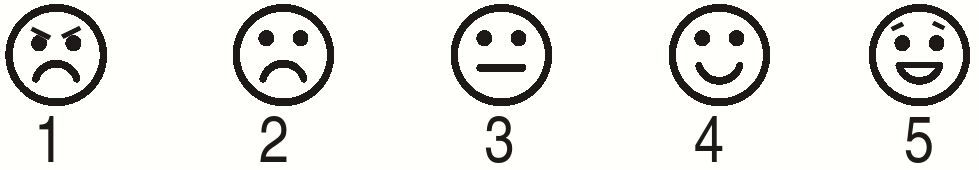
\includegraphics[width=0.40\textwidth]{HappinessMetric}
  \caption{Medida de satisfacción}
  \centering
  \label{fig:HappinessMetric} %\ref{fig:HappinessMetric}
  \end{figure}
  \FloatBarrier

  Otra escala para medir felicidad puede ser de siete puntos. Por ejemplo a la pregunta... ¿Cómo calificaría su felicidad en este momento? Se puede responder con 1 que es totalmente triste, 2 es muy triste , 3 es triste, 4 es ni feliz ni triste, 5 es bastante feliz, 6 es muy feliz y 7 es completamente feliz\footnote{\cite{U-K-University-2014}}.
  }
  
  \item {¿Qué va a hacer que me sienta mejor?}
  \end{enumerate}

Cuando tenemos la información de cada miembro del equipo, el equipo puede hacer una lluvia de ideas de cómo hacer para mejorar y aumentar la felicidad en el siguiente Sprint y darle curso y seguimiento a las acciones propuestas.

}

\item {\textbf{Team Morale:}
Indicador moral de equipo dice cómo está la moral en tu equipo. La moral del equipo es una medida más estable y confiable que la felicidad del equipo \footnote{Agile Teams: Don't use happiness metrics, measure Team Morale. Agilistic, Christiaan Verwijs, 2014.}. Esta métrica mide el orgullo, entusiasmo, energía, resiliencia, disposición para ayudarse mutuamente y motivación por el significado y propósito. Se puede medir mediante encuestas periódicas. Un cuestionario simple y práctico puede ser el siguiente (Las preguntas individuales se califican en una escala de 1 a 7 o de 1 a 5):
  \begin{enumerate}
  \item {¿Me siento bien (siento que encajo) y me siento fortalecido en mi equipo?}
  \item {¿Estoy orgulloso del trabajo que hago para mi equipo?}
  \item {¿Estoy entusiasmado con el trabajo que hago para mi equipo?}
  \item {¿Encuentro el trabajo que hago para mi equipo de significado y con propósito?}
  \end{enumerate}
}

\item {\textbf{Team Stability:} Se considera que se logra buena colaboración con equipos estables. Por ese motivo, bajo el marco ágil, se prioriza a los equipos estables por sobre los proyectos\footnote{The Disciplined Agile (DA) Framework}. Es decir que se recomienda mantener a los equipos estables y evitar mezclar personas entre equipos o desarmar equipos para asignar a otros proyectos (la rotación). Los equipos estables tienden a conocer mejor su capacidad, lo que permite cierta capacidad de predicción y mayor sinergia. Los miembros del equipo deben dedicarse a un solo equipo siempre que sea posible. Pero esto no siempre se logra por la rotación laboral o necesidades de la empresa. Por eso es útil medir el aspecto de “Team Stability” o  de rotación. Pues hay que mantener una rotación baja saludable.
}

\item {\textbf{Team Skill Balance:} 
Si existe un desbalance de conocimientos y de esfuerzo en el equipo puede provocar la fatiga de algunos integrantes, problemas por eslabones débiles (en contingencias, entrevistas, solución de problemas, etc.), dependencias sobre alguna persona o desavenencias por percepción de inequidad de esfuerzos. Un indicador de balance de competencias del equipo (Team Skill Balance Average) podría ayudar a que el equipo sea capaz de trabajar como una unidad integrada. Cada integrante debe ser un poco más multifuncional, colaborando en tareas o actividades que no son su fuerte o especialidad. 
}

\end{enumerate}

\subsection{Métricas del proceso de trabajo}

La entrega de valor fluida y continua es otro de los cuatro aspectos claves de la agilidad. Para mejorar este flujo de valor se busca, entre otras cosas, un flujo estable, sostenible y en un proceso de trabajo limpio (sin impedimentos ni desperdicios). En este sentido hay muchos indicadores clave del proceso de trabajo, de rendimiento, internos del equipo, que nos pueden ser de utilidad para monitorear el proceso de desarrollo y que nos permita la inspección y adaptación constante, como por ejemplo los siguientes\footnote{Scott y Jeff \cite{Scott-Jeff-2013} y la  Scrumalliance en un artículo llamado "Velocity, How to Calculate and Use Velocity to Help Your Team and Your Projects", por Catia Oliveira (6 February 2014).}:

\begin{enumerate}

\item {\textbf{Velocity:} La 'velocidad'\footnote{"Sum of original estimates of all accepted work" \cite{Scott-Jeff-2013}.} es el número de unidades de trabajo o puntos de historia SP estimados y aceptados por un equipo en una iteración Sprint. En otras palabras, es el conjunto de puntos de historia totales conseguidos (aceptados) por el equipo al final de cada Sprint\footnote{\cite{Jipson-Thomas-2015}}. Aquí hay que tener en cuenta que el Story Points o SP es una unidad de medida que indica una cantidad de alcance o trabajo que puede ser entregado o tamaño de producto estimado para entregar. Representa la complejidad o esfuerzo necesario para terminar las tareas de una historia \footnote{\cite{Jipson-Thomas-2015}}. El SP sirve como estimación de la complejidad en forma relativa y sumativa que hacen los desarrolladores. También hay que tener en cuenta que es una unidad subjetiva que depende de qué equipo hace la estimación de medida.} 

Esta definición es la clásica y es algo genérica. Hay tres formas más específicas de interpretar y medir la velocidad:

  \begin{enumerate}

  \item{\textbf{Velocidad de trabajo:} cuando la velocidad muestra la cantidad de trabajo o funcionalidad que un equipo entrega (aceptada) en un sprint\footnote{"Velocidad en la que el equipo pueda completar el trabajo en un Sprint, número de funcionalidades entregadas en un sólo Sprint o Número de Story Points hecho en un determinado Sprint" \cite{SBOK-2013}}, incluyendo las de valor indirecto. En este sentido, las historias de usuarios completadas (tomadas del backlog técnico) que tienen valor indirecto para el cliente, las correcciones de errores, deuda técnica, migraciones y refactorizaciones sí cuentan en la velocidad. En este caso, la velocidad del equipo da pocas indicaciones sobre el verdadero valor de negocio entregado y más sobre la capacidad que puede producir. Pues la velocidad, en este sentido, no suele tener relación directa con el valor de negocio entregado. Como no se suele aclarar bien la definición de velocidad se suele entender que se trata de esta perspectiva pero, sin embargo, en Scrum clásico se sobreentiende que los equipos deben entregar valor de punta a punta, por lo que la velocidad debería estar ligada al valor como la siguiente definición.
  }

  \item{\textbf{Velocity en nueva funcionalidad:} cuando la velocidad muestra solo la cantidad de funcionalidad de valor para el negocio que un equipo entrega (aceptada) en un sprint. En este sentido, las historias de usuarios que no tienen ningún valor para el cliente o incompletas, las correcciones de errores y las refactorizaciones no cuentan en la velocidad\footnote{\cite{David-Koontz-2014}}. En este caso, la velocidad del equipo da un indicio sobre el valor de negocio entregado por el equipo. En Scrum original o clásico se sobre-entiende que las historias son las que aportan valor, por tal motivo a veces no se aclara explícitamente esto.
  }
  
  \item{\textbf{Value Velocity:} es una forma interesante para medir la productividad (sugerida por James Shore\footnote{\cite{James-Shore-2015}}) similar a la velocidad tradicional o velocidad de trabajo, excepto que se basa en estimaciones de valor de negocio (Business Value Point) hechas por el PO antes de la planeación.
  }
  
  \end{enumerate}

\item {\textbf{Average Velocity:} De la velocity de cada Sprint se calcula la velocidad promedio o "Average Velocity" que es el número de unidades de trabajo o SP promedio estimados y aceptados por un equipo en un conjunto de iteraciones Sprint. En un equipo ágil de velocidad estable, la velocidad promedio (por ejemplo de los últimos 4 Sprints) es un indicador adelantado de la velocidad estimada para el próximo Sprint (bajo las mismas condiciones de los Sprints usados para calcularla).}

\item {\textbf{Work Capacity:} La Capacidad es la suma de todos los trabajos reportados durante el Sprint, esten terminados o no\footnote{Scott y Jeff \cite{Scott-Jeff-2013}}. La capacidad es generalmente igual o superior a la Velocity. Aunque la Capacidad puede, en raras ocasiones, caer por debajo de la velocidad. Esto se debe a que la velocidad se calcula en base a las estimaciones originales de trabajo, mientras que la capacidad se calcula en base a la suma de trabajo real reportado\footnote{Scott y Jeff \cite{Scott-Jeff-2013}}. Por lo que en el caso de que esto suceda, lo que indica es que el equipo ha sobre estimado la complejidad de los trabajos solicitados. También existen otras formas de calcular o entender la capacidad. Por ejemplo:

  \begin{enumerate}
  
  \item {\textbf{Capacidad en puntos ideales:} La capacidad puede ser una idealización basada en la velocidad promedio, o sea, los puntos de la historia que se pueden considerar gastar en la próxima carrera de velocidad.\footnote{\cite{Satish-Thatte-2013}}}

  \item {\textbf{Capacidad en horas:} La capacidad puede ser calculada en horas basados en la cantidad de miembros y la cantidad de horas efectivas de trabajo en un Sprint. Por ejemplo en un equipo de 8 miembros, con 6 horas de trabajo efectivo y un Sprint de 10 días, la capacidad en horas es igual a 480 hs (8 x 6 hs x 10).}

  \end{enumerate}

Cuando se definió el marco de trabajo, como algo mínimo de cosas para que funcione, se dejó lo más simple posible. Debido a ello, el concepto de Velocity sí es partes del marco de trabajo, pero Working capacity no lo es, aunque es ampliamente usado \footnote{Erich Buhler, Agilib.org 2015, Proyecto Mercury 2015 (LAN), \cite{Erich-Buhler-Coach-2015}.}.
}

\item {\textbf{Focus Factor:} El factor de foco revela el foco que el equipo ha tenido para entregar valor y su prestancia. El mismo es la relación entre la Velocity y la capacidad de trabajo: ( Velocity / Work Capacity ) x 100\%. La misma debe permanecer en la vecindad de 80 \% en promedio para un equipo saludable. Estos puntos de datos por debajo del 80 por ciento indican un equipo que está interrumpido o incapaz de convertir su trabajo estimado en trabajo aceptado mostrando poca previsibilidad. Cuando el valor es alto, cercano al 100, el equipo ha estado bajo la previsión de su capacidad, aunque esto no indica necesariamente que están trabajando bien. Por ejemplo, el equipo puede estar aparentando ser perfecto forzando la coincidencia.}

\item {\textbf{Targeted Value Increase (TVI+)} El TVI+ responde a cuánto cambio ha habido en la velocidad del equipo a través del tiempo desde el primer Sprint. Es la Velocity del Sprint actual dividido la Velocity Original (velocity del primer sprint): ( Current Sprint’s Velocity / Original Velocity ) x 100\%. Sirve para medir el aumento de la contribución de valor de un equipo en base a su velocidad origen Sprint a Sprint.
Por ejemplo, si el resultado es 200\% significa que el equipo ha duplicado su capacidad de resolver con éxito la complejidad requerida.
}

%Otras: Percentage of Adopted Work, Percentage of Found Work, Accuracy of Estimation, Accuracy of Forecast, Targeted Value Increase (TVI+), Success at Scale

\item {\textbf{Delivery rate:}
La tasa de entrega es un indicador que nos puede servir para ver la evolución de los tiempos de entrega. Nos puede ayudar a mejorar el continuous delivery.
}

\end{enumerate}

\subsection{Métricas de Calidad de Producto}

Bajo el marco ágil buscamos la excelencia técnica y en esa vía buscamos productos de calidad excelente. Pues bien, como se imaginan, tendremos que medir de algún modo la calidad de nuestro producto, ya sea calidad interna o del producto operando. Podemos citar algunos indicadores.

  \begin{enumerate}    

  \item {\textbf{Test Coverage:} La cobertura de prueba es una herramienta útil para encontrar partes no probadas de una base de código, lo cual nos ayuda a saber si se están realizando pruebas suficientes para apoyar el aseguramiento de calidad.
}

  \item {\textbf{Escaped defects:}
Un defecto escapado es un defecto que no fue encontrado por el equipo en el proceso de desarrollo y que escapó al control de calidad interno del equipo. Por lo general, esos problemas son incidentes en operaciones (OPCON), es decir que los encuentran los usuarios finales una vez que la versión de release fue publicada y puesta a su disposición. Su cálculo más simple es cantidad en un período dado (por ejemplo cantidad de OPCON por sprint).
}

  \item {\textbf{Performance:}
Las métricas de prestancia o rendimiento de aplicación nos ayudan a detectar problemas o posibles mejoras. En el caso de aplicaciones web hay una infinidad de indicadores que se pueden usar (“Fiability”, “Uptime”, “Loading time”, “Average Application Response Time”, “Peak Response Time”, “Error Rate”). El equipo debe elegir los necesarios para el contexto de operatividad y objetivos de negocio.
}

  \end{enumerate}

\subsection{Métricas de impacto de negocio}

Siguiendo una de las claves de la agilidad, el flujo de entrega de valor continuo, es que podemos suponer que la verdadera medida de éxito en Scrum es el incremento de producto que es valioso para el cliente, para entregar valor de forma temprana. Pero… ¿Cómo medir qué es valioso para el cliente?
Scrum no prescribe métricas de negocio o indicadores clave de impacto de negocio, aunque es necesario usarlos para saber si estamos entregando valor o generando el impacto deseado. El PO tiene el poder de tomar la decisión última de negocio y necesita datos empíricos para hacerlo. Además, en el proceso de inspección y adaptación, para construir el producto adecuado, el equipo con el PO necesitan observar indicadores de producto, orientarse, decidir y actuar, en busca de maximizar el valor. En esta vía, el PO tiene la posibilidad de usar Business Value Point para estimar valor entregado o hacer una distinción entre historias de usuario de cara a cliente o técnicas (más adelante explicado). Por otro lado también se pueden manejar un conjunto mínimo y suficiente de indicadores de negocio. A estos indicadores se los suele llamar KPI's y en el caso de negocio podemos interpretarlos como indicadores claves de impacto del producto. Algunos son los siguientes.



  \begin{description}    

  \item {\textbf{Business Value Delivered:} Valor de negocio entregado. Se pueden contabilizar los Business Value o BV entregados en cada Sprint. El VB es el valor añadido que la feature/historia aporta al negocio\footnote{\cite{Pointet-Botton-2012}}. A semejanza del SP, el Business Value Point o BVP sirve como estimación del valor de negocio en forma relativa y sumativa que hace el PO. También hay que tener en cuenta que es una unidad subjetiva que depende de qué PO o equipo de personas hace la estimación de medida.
} 
 
  \item {\textbf{SHSAT:} Grado de satisfacción de los Stakeholders. Se puede medir la felicidad de los Stakeholder como indicador de grado de satisfacción que indica qué tan contentos estuvieron con los resultados del Sprint y con la Review. Este relevamiento relacionado a la percepción de valor entregado se puede hacer en la misma Review.
}

  \item {\textbf{CSAT:} Customer Satisfaction es el índice de grado de satisfacción de los usuarios o clientes. Porcentaje de usuarios que respondieron "sí" para encontrar el servicio o producto útil en la encuesta de comentarios en comparación con el número total de encuestados.
}

  \item {\textbf{NPS:} El Puntaje Neto de Promotores (Net Promoter Score) mide la lealtad general de los clientes hacia un producto o servicio (fidelización). Mide qué probabilidades hay de que el cliente recomiende la compañía y, de forma indirecta, la propensión del consumidor a seguir siéndolo y resistir irse a la competencia.
}

  \item {\textbf{Cost Savings:} Grado de disminución de costos.
}

  \item {\textbf{Revenue:} Beneficios obtenidos.
}

  \item {\textbf{Completion rate:} La tasa de finalización mide el porcentaje de usuarios que finaliza con éxito o generan un resultado exitosamente. Se calcula dividiendo el número total de interacciones completadas con éxito por el número total de interacciones iniciadas. También se puede conocer como Funne o Full Compliance.
}

  \item {\textbf{Volume of Use:} Cuantos usuarios usan nuestra aplicación.
}
  \item {\textbf{Penetration:} Cuantos usuarios, de los que ya son clientes, usan nuestra aplicación del volumen total que usan dicho servicio en relación a todos los canales. Esto marca la parte del “Volume of Use” que crece por que los usuarios dejan de usar otros canales.
}

  \item {\textbf{Digital take-up:} Tasa de adopción para el servicio digital \footnote{Performance Dashboard del gobierno de australia (dashboard.gov.au)}.
}

  \item {\textbf{Market Share:} Cuantos usuarios, de los usuarios que no son clientes, fueron captados. O sea, que cantidad de usuarios nuevos captados de la competencia o del mercado. Esto marca si el “Volume of Use” crece por captación de nuevos usuarios.
}

  \begin{figure}[h]
  \centering
  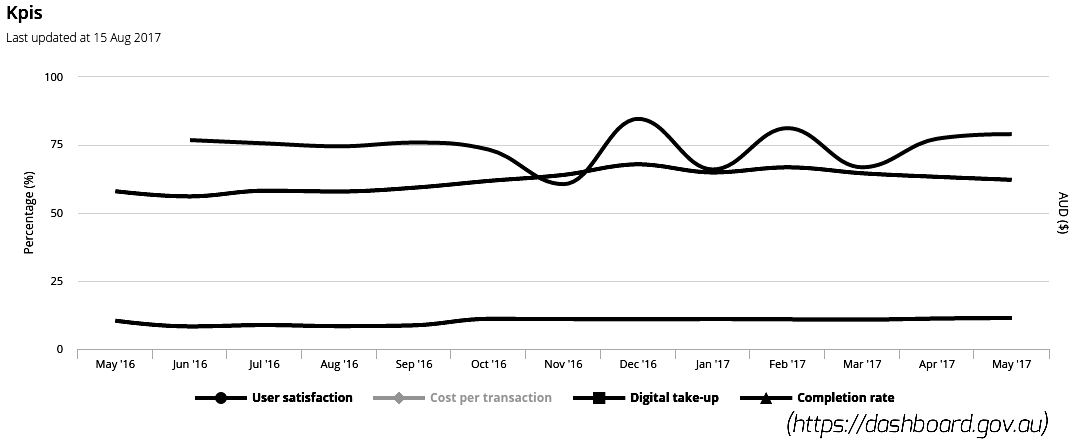
\includegraphics[width=0.99\textwidth]{kpis_dashboard_gov_au}
  \caption{KPIs del dashboard del gobierno de australia}
  \centering
  \label{fig:kpis_dashboard_gov_au} %\ref{fig:kpis_dashboard_gov_au}
  \end{figure}
  \FloatBarrier
  
\end{description}

\subsection{Métricas ágiles}

Por último, hay que tener en cuenta que para que las métricas estén bajo un marco Scrum deben respetar los principios de la agilidad. La medida principal es el software funcionando. Las métricas deben ser un medio de comunicación efectiva e impulsar la transparencia. Deben servir al equipo para que se auto-organize en procesos de corrección de desvíos y mejora contínua, apoyando la reflexión sobre cómo ser más efectivos. Y, principalmente, se debe buscar siempre la simplicidad. Las métricas que agregan complejidad innecesaria o sobre-información no son acordes a la agilidad. Lo difícil es encontrar el equilibrio entre un Scrum minimalista y hacer ingeniería. Si no medimos no podemos hacer análisis del sistema de trabajo, o sistema productivo, para mejorar con datos empíricos como lo requiere el trabajo ingenieril; pero si medimos excesivamente podemos estar generando desperdicio (burocracia y trabajo no relevante) y ruido informativo (datos que no generan información útil). Los KPI's no se deben convertir en objetivos que deben lograrse ni en herramienta de control de empleados.
